% =========================================================
% doc3-duality.tex — Section 3: The Duality Induced by Polarity
% Narrative: motivation / reflection / generation / integration /
% fundamental theorem / interpretation. Technical content from
% doc3-structures.tex, reorganized into a single argumentative flow.
% =========================================================

\section{The Duality Induced by Polarity}\label{sec:arch}

Section~\ref{sec:ps} established that a primitive polarity exists, is
logically independent of the semiring axioms, and is nontrivial on every
nontrivial model. It did not, however, reveal what the polarity produces.
The guiding question of the present section is therefore the following: does
a primitive polarity merely define an involution, or does it determine a
richer algebraic structure? We answer it in the affirmative, and the answer
unfolds in three consecutive steps. First the polarity reflects each
primitive operation into a dual operation; then the reflected operations are
shown to form a genuine semiring; finally the compatibility axiom
\eqref{ax:PJ} forces the primal and dual semirings to share a single order.
The hero of the section is thus not the polarity itself but the duality it
generates. Figure~\ref{fig:architecture} records the modules involved and
the axioms that link them.

% Two scale parameters: physical size per grid unit.
\def\xunit{0.8cm}
\def\yunit{0.5cm}

\begin{figure}[ht]
\centering
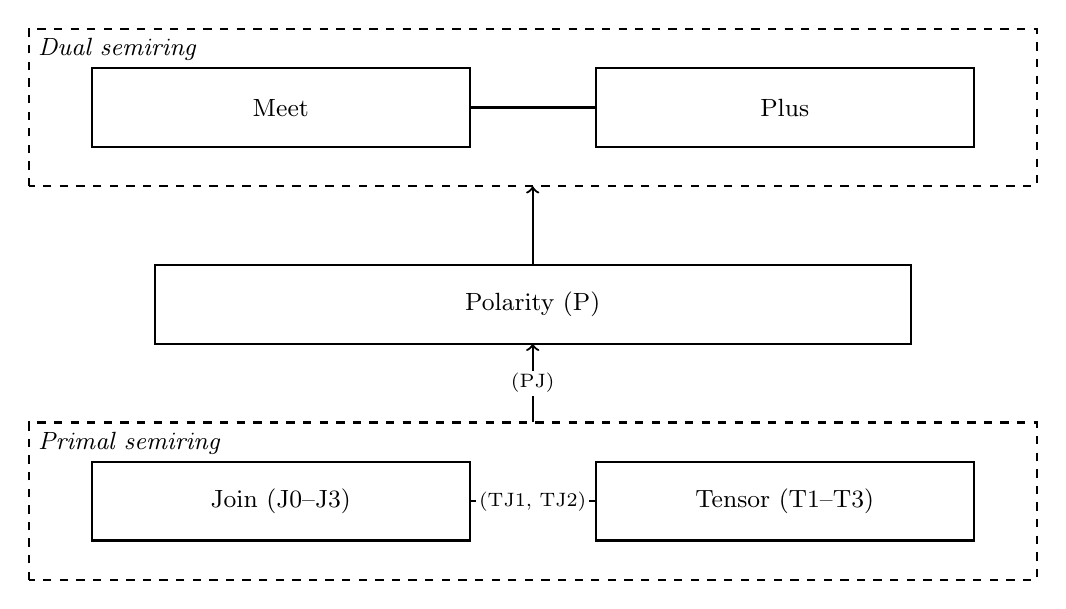
\begin{tikzpicture}[x=\xunit, y=\yunit, thick, font=\small]

% ---- Primal semiring: outer box (0,0) to (16,4) ----
\draw[dashed] (0,0) rectangle (16,4);
\node[anchor=north west, inner sep=3pt] at (0,4) {\itshape Primal semiring};
\draw (1,1) rectangle (7,3);
\node[align=center] at (4,2) {Join (J0--J3)};
\draw (9,1) rectangle (15,3);
\node[align=center] at (12,2) {Tensor (T1--T3)};
\draw (7,2) -- (9,2);
\node[fill=white, inner sep=1pt] at (8,2) {\scriptsize (TJ1, TJ2)};

% ---- Polarity: BL (2,6) TR (14,8), center (8,7) ----
\draw (2,6) rectangle (14,8);
\node at (8,7) {Polarity $(\mathrm{P})$};

% ---- Dual semiring: outer box (0,10) to (16,14) ----
\draw[dashed] (0,10) rectangle (16,14);
\node[anchor=north west, inner sep=3pt] at (0,14) {\itshape Dual semiring};
\draw (1,11) rectangle (7,13);
\node at (4,12) {Meet};
\draw (9,11) rectangle (15,13);
\node at (12,12) {Plus};
\draw (7,12) -- (9,12);

% ---- vertical links ----
\draw[->] (8,4) -- (8,6) node[midway, fill=white, inner sep=1pt] {\scriptsize (PJ)};
\draw[->] (8,8) -- (8,10);

\end{tikzpicture}
\caption{The modules of a PS. The primal semiring
$(X,\vee,\otimes,\ev,\eo)$ and its dual $(X,\wedge,\oplus,\ew,\ep)$ are
related through the polarity, which supplies axioms \eqref{ax:P} and
\eqref{ax:PJ}.}
\label{fig:architecture}
\end{figure}




\textcolor{blue}{we should reorganize:\\
Part 1 semiring --> idem com monoidal sinh order\\
Part2 add involution --> dual idem com semiring --> weak antitone\\
Part3 add PJ ---> merging 2 orders --> generate lattice.\\
Main Theorem: polar semiring generates polar semiring dual and antitone.}




\textcolor{blue}{Part 2 add involution}
The first step is reflection. We introduce the operations conjugate to the
primitive ones and record their basic laws; nothing beyond the involution
axiom \eqref{ax:P} is used.

\begin{definition}[Derived operations and meet order]\label{def:derived}
Let $(X,\vee,\otimes,{}^{*},\ev,\eo)$ be a PS. Define the \emph{meet}, the
\emph{plus}, and the derived units by
\begin{equation}\label{eq:derived-ops}
  a \wedge b := \dstar{(\dstar{a} \vee \dstar{b})},\qquad
  a \oplus b := \dstar{(\dstar{a} \otimes \dstar{b})},\qquad
  \ew := \dstar{\ev},\qquad
  \ep := \dstar{\eo},
\end{equation}
and the \emph{meet order} by
\begin{equation}\label{eq:meet-order}
  a \leqm b \;:\Longleftrightarrow\; a \wedge b = a.
\end{equation}
\end{definition}

A word on terminology fixes the two levels at which the involution operates.
Following the historical order of the two notions, with involutions
belonging to pure algebra and polarities to order theory
\citep{Birkhoff1940}, we call a structure \emph{involutive} when it satisfies
only $\dstar{(\dstar{a})} = a$, and reserve the adjective \emph{polar} for
structures in which the involution is additionally compatible with the
induced order via \eqref{ax:PJ}. The reflection step lives entirely at the
involutive level: no order is required for it. The duality laws below are the
De Morgan identities relating the primitive operations to their conjugates.

\begin{proposition}[Duality laws]\label{prop:duality}
Let $(X,\vee,\ev)$ and $(X,\otimes,\eo)$ be commutative monoids and let
${}^{*}$ satisfy \eqref{ax:P}. With the derived operations
\eqref{eq:derived-ops}, the following hold for all $a,b \in X$:
\begin{align}
  \dstar{(a \wedge b)} &= \dstar{a} \vee \dstar{b}, \label{eq:RD1}\\
  \dstar{(a \oplus b)} &= \dstar{a} \otimes \dstar{b}, \label{eq:RD2}\\
  \dstar{(a \vee b)} &= \dstar{a} \wedge \dstar{b}, \label{eq:RD3}\\
  \dstar{(a \otimes b)} &= \dstar{a} \oplus \dstar{b}, \label{eq:RD4}\\
  \dstar{\ev} = \ew,\quad \dstar{\ew} = \ev,&\quad
  \dstar{\eo} = \ep,\quad \dstar{\ep} = \eo. \label{eq:RD5}
\end{align}
\end{proposition}

\begin{proof}
For \eqref{eq:RD1}, apply \eqref{ax:P} to the definition:
$\dstar{(a \wedge b)}
 = \dstar{(\dstar{(\dstar{a} \vee \dstar{b})})}
 = \dstar{a} \vee \dstar{b}$.
For \eqref{eq:RD3},
$\dstar{a} \wedge \dstar{b}
 = \dstar{(\dstar{(\dstar{a})} \vee \dstar{(\dstar{b})})}
 = \dstar{(a \vee b)}$ by \eqref{ax:P}. Equations \eqref{eq:RD2} and
\eqref{eq:RD4} are the same computations with $\otimes,\oplus$ in place of
$\vee,\wedge$. In \eqref{eq:RD5}, the first and third equations are the
definitions in \eqref{eq:derived-ops}, and the other two follow by
\eqref{ax:P}.
\end{proof}

% \begin{proposition}[Reflected modules]\label{prop:reflected-modules}
% Under the hypotheses of \Cref{prop:duality}, $(X,\wedge,\ew)$ and
% $(X,\oplus,\ep)$ are commutative monoids, and if \eqref{ax:J0} holds then
% $\wedge$ is idempotent.
% \end{proposition}

% \begin{proof}

% \end{proof}

The polarity reflects every primitive object into a dual one, and
does so at no axiomatic cost beyond \eqref{ax:P}. This yields a candidate
dual semiring $(X,\wedge,\oplus,\ew,\ep)$, though at this stage only its two
monoid modules have been secured; the axioms linking them remain to be
verified. That is the second step, generation, and it too uses only
\eqref{ax:P}: the linking axioms of the dual are the reflections of the
linking axioms of the primal.

\begin{proposition}[Dual PS]\label{prop:dual-semiring}
Let $(X,\vee,\otimes,{}^{*},\ev,\eo)$ be a PS.
Then $(X,\wedge,\oplus,*, \ew,\ep)$
is also a PS.
\end{proposition}

\begin{proof}
Commutativity of $\wedge$ is immediate from \eqref{ax:J2}. For associativity,
using \eqref{eq:RD1},
$$
  (a \wedge b) \wedge c
  = \dstar{\bigl(\dstar{(a \wedge b)} \vee \dstar{c}\bigr)}
  = \dstar{\bigl((\dstar{a} \vee \dstar{b}) \vee \dstar{c}\bigr)},
$$
and \eqref{ax:J1} reassociates the inner join; reversing the steps gives
$a \wedge (b \wedge c)$. For the unit,
$a \wedge \ew
 = \dstar{(\dstar{a} \vee \dstar{\ew})}
 = \dstar{(\dstar{a} \vee \ev)}
 = \dstar{(\dstar{a})} = a$
by \eqref{eq:RD5}, \eqref{ax:J3}, and \eqref{ax:P}. The plus module is the
same argument with \eqref{ax:T1} to \eqref{ax:T3}. Idempotence is
$a \wedge a = \dstar{(\dstar{a} \vee \dstar{a})} = \dstar{(\dstar{a})} = a$
by \eqref{ax:J0} and \eqref{ax:P}.

Axioms \eqref{ax:J0} to \eqref{ax:J3} for $\wedge$ and \eqref{ax:T1} to
\eqref{ax:T3} for $\oplus$ are \Cref{prop:reflected-modules}. For the dual of
\eqref{ax:TJ1}, using \eqref{eq:RD1} to \eqref{eq:RD4} and \eqref{ax:TJ1} in
the primal,
$$
  a \oplus (b \wedge c)
  = \dstar{\bigl(\dstar{a} \otimes (\dstar{b} \vee \dstar{c})\bigr)}
  = \dstar{\bigl((\dstar{a} \otimes \dstar{b}) \vee
                 (\dstar{a} \otimes \dstar{c})\bigr)}
  = (a \oplus b) \wedge (a \oplus c).
$$
For the dual of \eqref{ax:TJ2},
$a \oplus \ew = \dstar{(\dstar{a} \otimes \ev)} = \dstar{\ev} = \ew$
by \eqref{eq:RD5} and \eqref{ax:TJ2}. Hence all nine semiring axioms hold for
the dual operations.
\end{proof}

Every PS thus canonically induces a dual semiring, the first principal result
of the section. The two semirings, however, have so far been produced side by
side, each with its own order, and it is natural to ask whether they are
independent. The third step, integration, shows that they are not: the single
axiom \eqref{ax:PJ}, the one axiom relating the polarity to the join and the
only one not yet used, welds the two together. We first record that the
tensor is monotone, which the integration will need on the dual side.



\textcolor{blue}{Part 3 order}

\textcolor{blue}{Part 1 semiring --> idem com monoidal sinh order}

First we shoulde notice that $(X, \vee, e_\vee)$ is an idempotent commutative monoidal, thus it induces an order $\leq$ defined by 
\begin{equation*}
    a \leq b \Leftrightarrow a \vee b = b.
\end{equation*}
This order clearly satisfies reflexivity, antisymmetry and transitivity according to \eqref{ax:J0}-\eqref{ax:J3}.

Since $(X, \wedge,1_\wedge)$ is an idempotent comutative monoidal, we may define 
\begin{equation*}
    a \leq^* b \Leftrightarrow a \wedge b = a.
\end{equation*}

By the definitions of these two orders, we have 
\begin{lemma}\label{lem:tensor-monotone}
For $a \leq b$ and $p\leq^* q$, we have
\begin{enumerate}
    \item $a \vee c \leq b \vee c$
    \item $a \otimes c \leq b \otimes c$
    \item $p \wedge c \leq^* q \wedge c$
    \item $p \oplus c \leq^* q \oplus c$
\end{enumerate}
\end{lemma}

\begin{proof}
If $a \vee b = b$, then by \eqref{ax:TJ1} and \eqref{ax:T2},
$(a \otimes c) \vee (b \otimes c) = (a \vee b) \otimes c = b \otimes c$.
\end{proof}

By definition of $\leq$ and $\leq^*$, we have 
$$a \leq b \iff \dstar{b} \leqm \dstar{a}.$$
It means that the antitone of polarity comes from the definition of orders we define.
In the following, we show that, the \eqref{ax:PJ} axiom is actualy equivalent to the fact that the two orders coincide
$$\leq \equiv \leq^*.$$
This makes the antitone of polarity happens on a single poset.

\begin{proposition}[Order compatibility]\label{prop:order-compat}
In the presence of the other ten axioms, the following are equivalent to \eqref{ax:PJ}
\begin{enumerate}
  \item $a \vee b = b \iff a \wedge b = a$;
  \item $a \leq b \iff \dstar{b} \leq \dstar{a}$;
  \item $a \wedge (a \vee b) = a$ and
        $a \vee (a \wedge b) = a$.
\end{enumerate}
The last equalities are known as the absorption laws of join and meet.
\end{proposition}

\begin{proof}
(1)$\Leftrightarrow$(2): by \eqref{eq:derived-ops} and \eqref{ax:P},
$b \wedge a = a$ holds if and only if
$\dstar{(\dstar{b} \vee \dstar{a})} = a$, if and only if
$\dstar{b} \vee \dstar{a} = \dstar{a}$; so (2) is a literal restatement of
(1).

(1)$\Leftrightarrow$(3): unfolding \eqref{eq:meet-order},
$\dstar{b} \leqm \dstar{a}$ means $\dstar{b} \wedge \dstar{a} = \dstar{b}$,
that is, $\dstar{(b \vee a)} = \dstar{b}$ by \eqref{eq:RD3}, that is,
$b \vee a = a$ by injectivity of ${}^{*}$; renaming the variables shows (3) to
be a restatement of (1).

(2)$\Rightarrow$(4): since $a \leq a \vee b$ by \eqref{ax:J0} and
\eqref{ax:J1}, item (2) yields $(a \vee b) \wedge a = a$, the first
absorption law. For the second, apply (2) in the direction
$b \wedge a = a \Rightarrow a \vee b = b$ to the pair $(a \wedge b, a)$: since
$a \wedge (a \wedge b) = a \wedge b$ by \Cref{prop:reflected-modules}, one has
$(a \wedge b) \vee a = a$.

(4)$\Rightarrow$(2): if $a \vee b = b$, then
$a \wedge b = a \wedge (a \vee b) = a$, so $b \wedge a = a$. Conversely, if
$b \wedge a = a$, then $a \vee b = (b \wedge a) \vee b = b$ by the second
absorption law and commutativity.
\end{proof}

\begin{proposition}[Order structure]\label{prop:order-structure}
In any PS:
\begin{enumerate}
%   \item $\leq$ is a partial order and $\leq \;=\; \leqm$;
  \item $\ev \leq a \leq \ew$ for all $a$;
%   \item $a \leq b$ implies $a \wedge c \leq b \wedge c$ and
%         $a \oplus c \leq b \oplus c$;
  \item $(X,\vee,\wedge)$ is a bounded, possibly non-distributive lattice.
\end{enumerate}
\end{proposition}

\begin{proof}
(1) That $\leq$ is a partial order was noted in Section~\ref{sec:ps}. By
\Cref{prop:order-compat}(2), $a \leq b$ if and only if $a \wedge b = a$, which
is $a \leqm b$; hence the two orders coincide.

(2) $\ev \leq a$ is \eqref{ax:J3} with \eqref{ax:J2}. For $a \leq \ew$:
by \eqref{ax:PJ} this is equivalent to
$\dstar{\ew} \vee \dstar{a} = \dstar{a}$, that is,
$\ev \vee \dstar{a} = \dstar{a}$, which holds by \eqref{ax:J3}.

(3) If $a \leq b$, then $a \wedge b = a$ by \Cref{prop:order-compat}(2), so
$(a \wedge c) \wedge (b \wedge c) = (a \wedge b) \wedge (c \wedge c)
 = a \wedge c$
by \Cref{prop:reflected-modules}, whence $a \wedge c \leqm b \wedge c$, and
(1) concludes. For $\oplus$: from $a \leq b$, \eqref{ax:PJ} gives
$\dstar{b} \leq \dstar{a}$, \Cref{lem:tensor-monotone} gives
$\dstar{b} \otimes \dstar{c} \leq \dstar{a} \otimes \dstar{c}$, and applying
\eqref{ax:PJ} once more with \eqref{eq:RD2} yields
$a \oplus c \leq b \oplus c$.

(4) The least-upper-bound property of $\vee$ is standard in idempotent
commutative monoids. For $\wedge$, dualize: by \eqref{ax:PJ} and
\eqref{eq:RD3}, the lower bounds of $\{a,b\}$ correspond under ${}^{*}$ to the
upper bounds of $\{\dstar{a},\dstar{b}\}$, and the correspondence sends
$a \wedge b$ to $\dstar{a} \vee \dstar{b}$; the greatest-lower-bound property
follows. The absorption laws of \Cref{prop:order-compat}(4) then exhibit
$(X,\vee,\wedge)$ as a lattice, bounded by (2). Distributivity of $\vee$ over
$\wedge$ is not asserted and indeed fails in general.
\noteAI{If you want a concrete non-distributive example here, add the diamond
$M_3$ with a suitable involution and check \eqref{ax:TJ1}--\eqref{ax:TJ2} for
a chosen tensor; otherwise the claim ``fails in general'' should be softened
or given a citation.}
\end{proof}

The join module together with \eqref{ax:P} and \eqref{ax:PJ} alone yields a
bounded, possibly non-distributive lattice carrying an antitone involution
that satisfies the De Morgan laws. We call such a structure a \emph{Polar
Lattice}; it coincides with the classical notion of a bounded i-lattice
\citep{Kalman1958}, an identification to which we return in
Section~\ref{sec:positioning}. The three steps now combine into the central
theorem of the section, which states that the induced duality is in fact a
self-duality.

\begin{theorem}[Fundamental Structure Theorem]\label{thm:fundamental}
Let $(X,\vee,\otimes,{}^{*},\ev,\eo)$ be a PS. Then the dual structure
$(X,\wedge,\oplus,{}^{*},\ew,\ep)$ is again a PS, the polarity
${}^{*}\colon X \to X$ is an isomorphism and antitone.
\end{theorem}

\begin{proof}
By \Cref{prop:dual-semiring} the dual reduct $(X,\wedge,\oplus,\ew,\ep)$ is a
primitive semiring, and axiom \eqref{ax:P} is unchanged under passage to the
dual. It remains to verify the dual of \eqref{ax:PJ}, namely
$a \wedge b = b \iff \dstar{b} \wedge \dstar{a} = \dstar{a}$; by
\Cref{prop:order-compat}(2) and \Cref{prop:order-structure}(1) both sides
translate into statements about $\leq$, namely $b \leq a$ on the left and
$\dstar{a} \leq \dstar{b}$ on the right, and these are equivalent by
\eqref{ax:PJ}. Thus the dual is a PS. The map ${}^{*}$ is a bijection by
\eqref{ax:P}, and \eqref{eq:RD3} to \eqref{eq:RD5} say exactly that it sends
$\vee$ to $\wedge$, $\otimes$ to $\oplus$, $\ev$ to $\ew$, and $\eo$ to
$\ep$; hence it is an isomorphism onto the dual. The coincidence of the two
orders is \Cref{prop:order-structure}(1).
\end{proof}

Section~\ref{sec:ps} proved that polarity can be taken as primitive; the
present section proves that, once primitive, polarity automatically generates
a complete dual architecture. Reflection produces the conjugate operations,
generation assembles them into a dual semiring, and integration fuses the two
semirings into a single self-dual structure, at which point applying the
construction twice returns the original PS, since $\dstar{(\dstar{a})} = a$.
What Section~\ref{sec:ps} presented as an isolated involution has become an
order-reversing isomorphism between a semiring and its dual, obtained from
three compatibility axioms and no residual. The natural question that remains
is where this generated duality sits among existing algebraic structures,
which is the subject of Section~\ref{sec:positioning}.


